\documentclass[entwurf]{uebblatt}

\begin{document}

\maketitle{6}

\begin{aufgabe}{Klassenzahlberechnungen}
\begin{enumerate}
\item Zeige, dass die quadratischen Zahlkörper~$\QQ[\sqrt{d}]$ für~$d \in \{
-7, -3, -2, -1, 2, 3, 5 \}$ die Klassenzahl~$1$ besitzen.
\item Zeige, dass auch~$\QQ[\sqrt{7}]$ die Klassenzahl~$1$ besitzt.
\item Was ist die Klassenzahl von~$\QQ[\sqrt{-5}]$?
\end{enumerate}
\end{aufgabe}

\begin{aufgabe}{Eine Schranke für die Diskriminante}
\begin{enumerate}
\item Sei~$K$ ein Zahlkörper vom Grad~$n$. Sei~$d_K$ die Diskriminante einer
Ganzheitsbasis. Zeige:
\[ |d_K| \geq (n^n / n!)^2 \cdot (\pi/4)^n. \]
\item Zeige: Bis auf~$\QQ$ selbst gibt es keinen Zahlkörper mit~$|d_K| = 1$.
\end{enumerate}
\end{aufgabe}

\begin{aufgabe}{Verzweigung von Primidealen}
\begin{enumerate}
\item Sei~$K = \QQ[\sqrt[3]{2}]$. Es ist~$(1,\sqrt[3]{2},\sqrt[3]{2}^2)$ eine
Ganzheitsbasis von~$\O_K$. Bestimme das Verzweigungsverhalten der
Primzahlen~$2, 3, 5$ und~$11$ in~$\O_K$.
\item Was möchte dir \emph{Mumfords Schatzkarte} mitteilen? Analysiere sie so
gut wie möglich!

\centering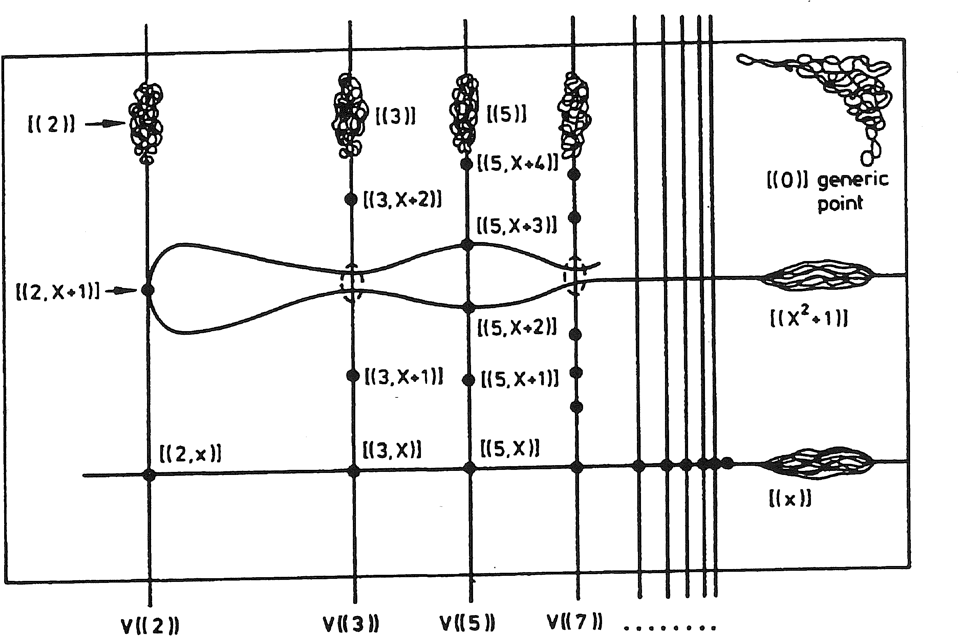
\includegraphics[width=0.7\textwidth]{images/mumfords-treasure-map}
\end{enumerate}
\end{aufgabe}

\end{document}
